
\documentclass[12pt]{article}
\usepackage{geometry} % see geometry.pdf on how to lay out the page. There's lots.
\usepackage{graphicx}
\geometry{a4paper} % or letter or a5paper or ... etc
% \geometry{landscape} % rotated page geometry

% See the ``Article customise'' template for come common customisations

\title{MADAI Workbench 1.8.0 Tutorial: \\A Supplement to the ParaView Tutorial}
\author{Cory Quammen}
\date{} % delete this line to display the current date

%%% BEGIN DOCUMENT
\begin{document}

\maketitle
\tableofcontents

\section{Introduction}

This tutorial will walk you through using several of the features of the MADAI Workbench. These features not available in a plain installation of ParaView.

The content of this tutorial assumes that you have gone through the ParaView Tutorial for version 3.98 or higher of ParaView.

\section{Ensemble Surface Slicing Representation}

In the ParaView tutorial, we have seen that several representations are available for displaying data in ParaView (3D Glyphs, Outline, Points, Surface, Surface with Edges, Wireframe). Another representation is suitable for displaying a group of surfaces using a technique called Ensemble Surface Slicing \cite{Oluwafemi2012}.

Open the files \texttt{apple.ply}, \texttt{banana.ply}, \texttt{cherry.ply}, and \texttt{grape.ply}. The Ensemble Surface Slicing representation operates on a set of surfaces grouped together into a multiblock dataset. To group the files, select them all in the Pipeline Browser by holding the shift key and selecting the first file in the browser and then the last. Next, group them together with Filters $\rightarrow$ Alphabetical $\rightarrow$ Group Datasets. The resulting display will show the union of the surfaces, the same as what you would get just by having all the surfaces' visibility turned on.

\begin{figure}[htbp]
   \centering
   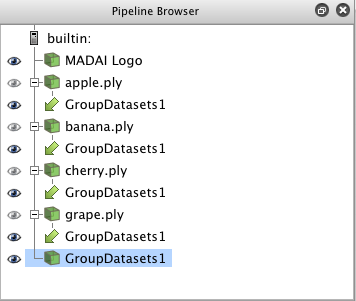
\includegraphics[scale=.5]{images/ESSGroupDatasets.png} % requires the graphicx package
   \caption{The fruit datasets \texttt{apple.ply}, \texttt{banana.ply}, \texttt{cherry.ply}, and \texttt{grape.ply} grouped together.}
   \label{fig:ESSGroupDatasets}
\end{figure}

Next, change the representation of the grouped surfaces to \textbf{Ensemble Surface Slicing}. Change the \textbf{Slice Width} setting to 2 and the \textbf{Plane Normal} to 0, 0, 1. You will now see all the surfaces, but slices will be taken out of each surface in such a way that shows all the surfaces.

\begin{figure}[htbp]
   \centering
   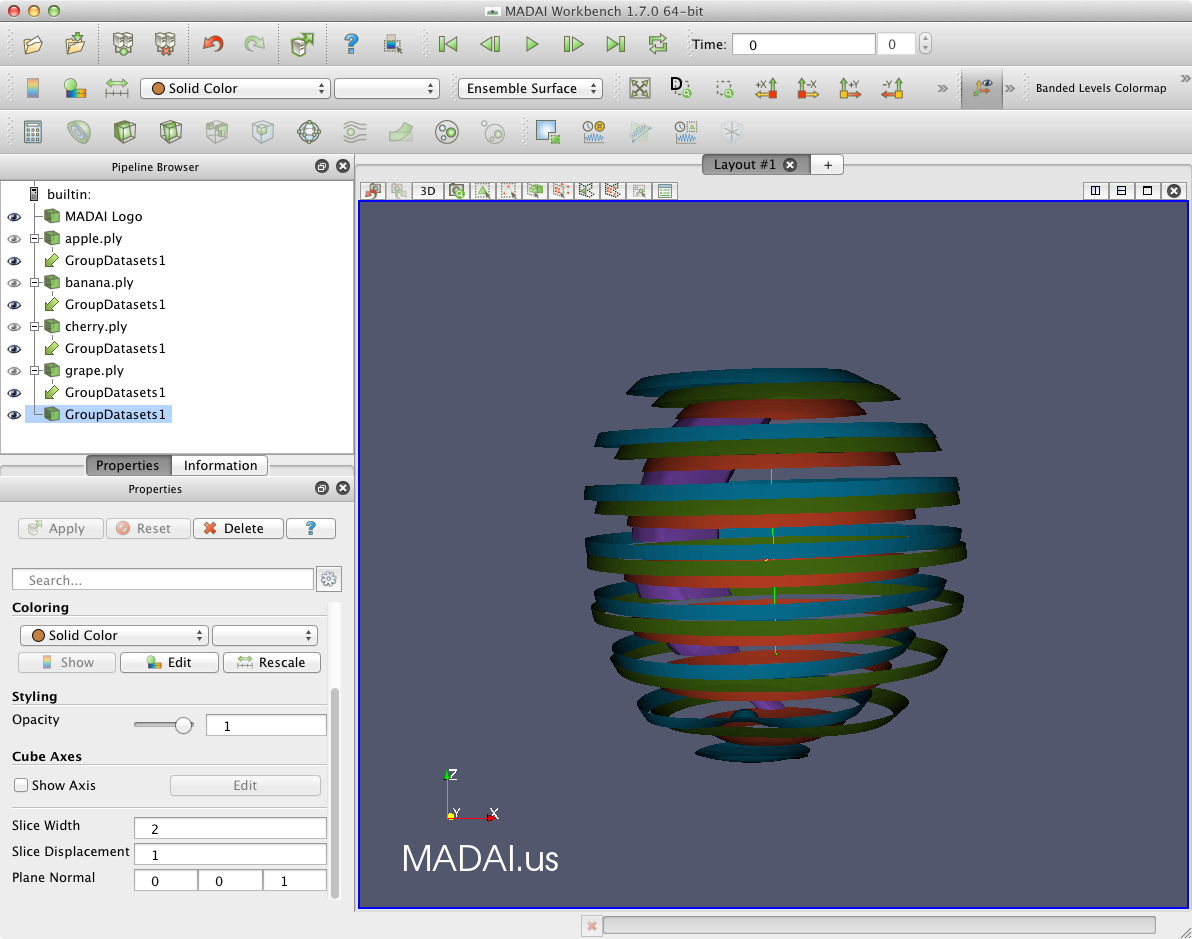
\includegraphics[scale=.25]{images/ESSSurfaces.png} % requires the graphicx package
   \caption{The fruit datasets displayed with the ensemble surface slicing technique.}
   \label{fig:ESSSurfaces}
\end{figure}

\section{Threshold Points Filter}

ParaView provides a Threshold filter that operates on cells in a dataset. Cells, such as triangle or tetrahedra, are elements that either have a surface area or volume. This is a problem when your dataset consists of points with no associated cells. This can show up in strange ways when you have applied a Threshold filter to your dataset, but no filtering appears to have been done.

To see that this is the case, create a point source by selecting Sources $\rightarrow$ Point Source. Change the \textbf{Number of Points} to 1000 and \textbf{Radius} to 1. Next, create a \textbf{Calculator} filter by selecting \textbf{Filters} $\rightarrow$ \textbf{Alphabetical} $\rightarrow$ \textbf{Calculator}. Set the \textbf{Result Array Name} to ``X'' and enter ``coordsX'' in the text field above the calculator buttons. This creates a point scalar field that has the same value as the x-coordinates of the points.

\begin{figure}[htbp]
   \centering
   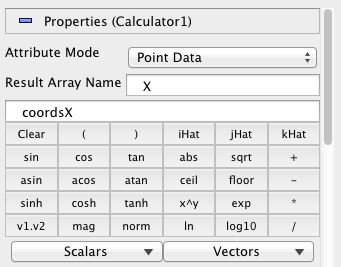
\includegraphics[scale=.5]{images/ThresholdPointsFilterCalculator.png} % requires the graphicx package
   \caption{Creating a point scalar field for the point data.}
   \label{fig:ThresholdPointsFilterCalculator}
\end{figure}

No apply the Threshold filter (Filters $\rightarrow$ Alphabetical $\rightarrow$ Threshold). Select ``X'' from the \textbf{Scalars} menu and uncheck the \textbf{All Scalars} checkbox and then click \textbf{Apply}. You should see all the original points. Next, change the \textbf{Maximum} value to 0.2. Again, all the original points are displayed, indicating that thresholding did not work. Select the \textbf{Calculator1} filter in the Pipeline Browser again and this time create a Threshold Points filter (Filters $\rightarrow$ Alphabetical $\rightarrow$ Threshold Points Filter). Select ``X'' as the scalars and change the right value of the \textbf{Threshold Range} to 0.2. This time, the points will be filtered such that points with the X value (and x-coordinate) above 0.2 are removed from the point set.

\begin{figure}[htbp]
   \centering
   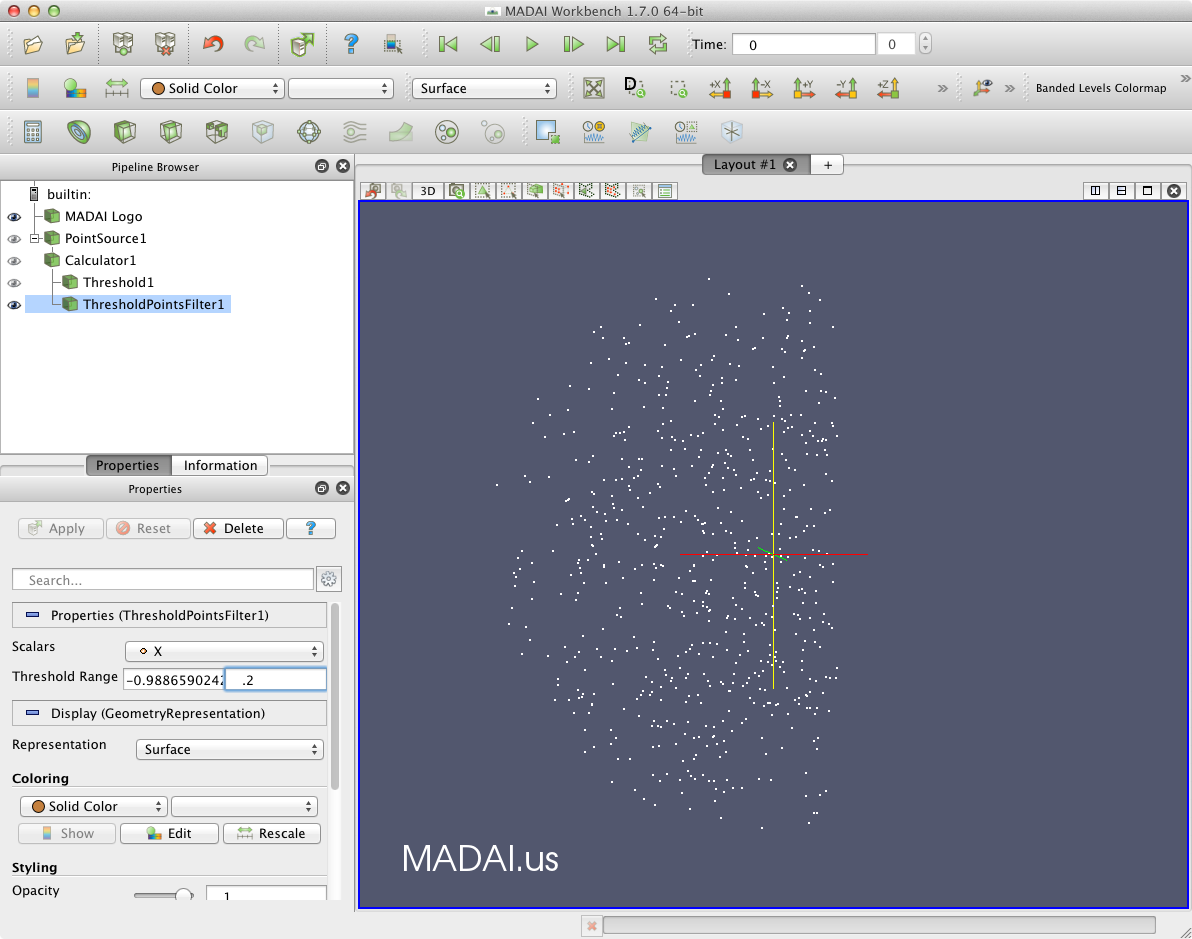
\includegraphics[scale=.25]{images/ThresholdPointsFilter.png} % requires the graphicx package
   \caption{Results of the \textbf{Threshold Points} filter.}
   \label{fig:ThresholdPointsFilter}
\end{figure}

\section{Binning Filter}

The Binning Filter provides a fast way to create a regular 2D or 3D grid representing density from a point set. If you have completed the exercise from the previous section, delete the Threshold1 and ThresholdPoints1 filters from the pipeline by right-clicking them and choosing the menu item \textbf{Delete}. Now click on the PointSource1 source and change the \textbf{Number of Points} to 100,000. Now apply a Binning filter to it (Filters $\rightarrow$ Alphabetical $\rightarrow$ Binning Filter). The default settings are fine. Click \textbf{Apply}. Now set the representation to \textbf{Slice} and set the \textbf{Slice Direction} to XY Plane. Move the \textbf{Slice} to the middle of the range. In the \textbf{Coloring} section, choose the \texttt{NumberDensity} point field in the popup menu and click the \textbf{Rescale} button.

\begin{figure}[htbp]
   \centering
   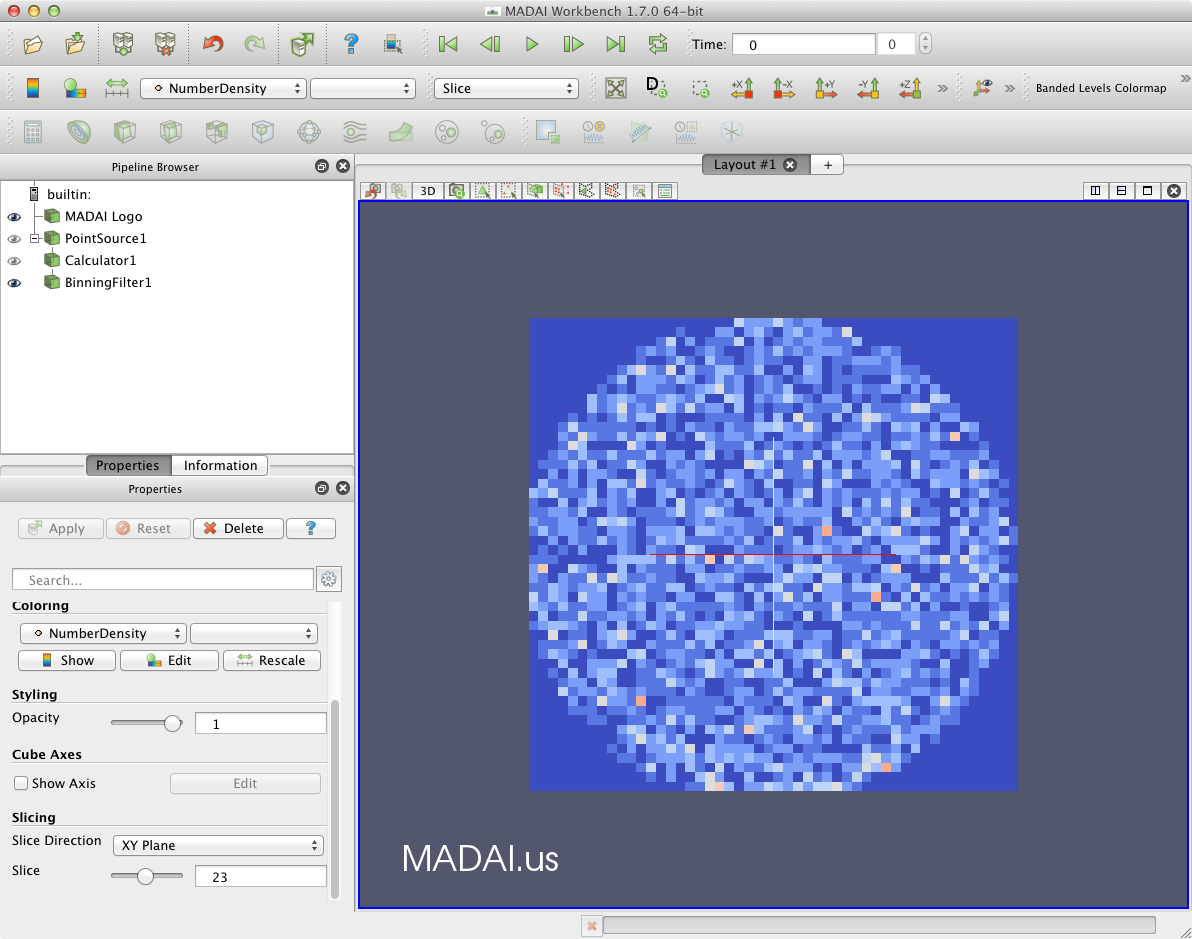
\includegraphics[scale=.25]{images/BinningFilter.png} % requires the graphicx package
   \caption{Results of the \textbf{Binning} filter.}
   \label{fig:BinningFilter}
\end{figure}

The \texttt{NumberDensity} feld gives the number of points that fall within each grid cell. In addition to the \texttt{NumberDensity} field, the binning filter also sums up each point data field. Change the point data field in the \textbf{Coloring} section to \texttt{X\_Density}. The value of each grid point in this filter's output is the sum of all the \texttt{X} values of the points that fall within the cell.

\begin{figure}[htbp]
   \centering
   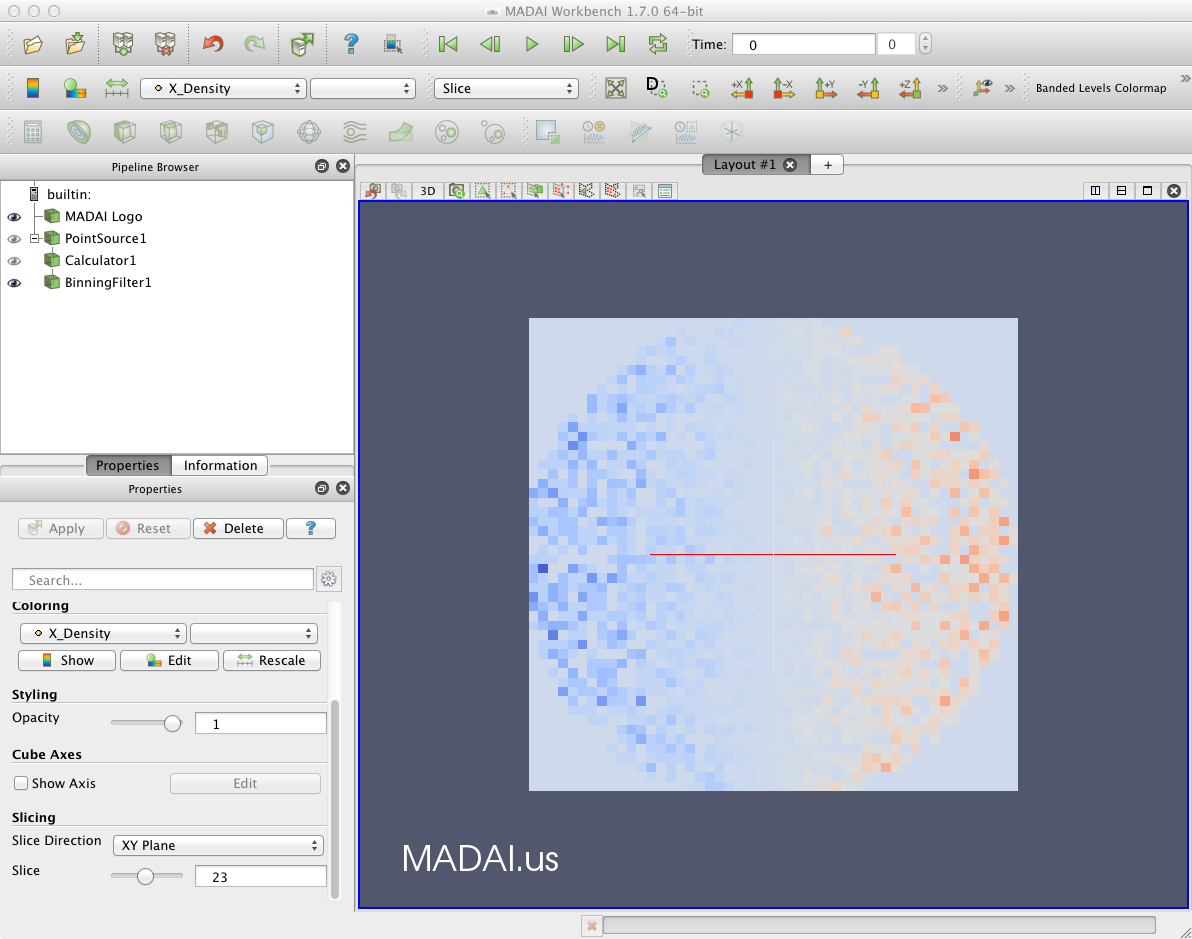
\includegraphics[scale=.25]{images/BinningFilter_XDensity.png} % requires the graphicx package
   \caption{The \texttt{X\_Density} field computed by the \textbf{Binning} filter from the \texttt{X} field.}
   \label{fig:BinningFilterXDensity}
\end{figure}

To get the average density of the points in the grid cel, you can divide the \texttt{X\_Density} field by the \texttt{NumberDensity} field. To do thisl, apply a \textbf{Calculator} filter to \texttt{BinningFilter1}, set the \textbf{Result Array Name} to \texttt{AverageX}, and set the text field to \texttt{X\_Density / NumberDensity}. 

\section{Gaussian Scalar Splatter Filter}

Whereas the Binning filter computes discrete summation of points within a grid cell, the Gaussian Scalar Splatter filter computes smoother density fields by spreading the values associated with each point according to an isotropic 3D Gaussian ``splat'' function whose integrated energy is 1. The 3D Gaussian splat has a size specified in units of standard deviation that determines how far the influence of each point reaches and how smooth the resulting scalar field. The splat is translated to each point in the input. The integrated portion of the splat that intersects a grid cell is computed and added to the value at the cell to arrive at a number density similar in concept to the number density field produced by the binning filter. In fact, this filter produces the same results as the binning filter as the size of the splat approaches 0. Each point data field \texttt{F} is multiplied by this integrated value and added to a new data field called \texttt{F\_Density}. An important feature of this filter is that if you integrate a dataset field produced by the filter and integrate the dataset field input to this filter, the answer is the same.

Add a Gaussian Scalar Splatter filter (Filters $\rightarrow$ MADAI $\rightarrow$ Gaussian Scalar Splatter) to Calculator. Leave the \textbf{Standard Deviation} setting at 0.1, but change the \textbf{Sample Dimensions} to 50 50 11. Click the \textbf{Apply} button. Next, change the representation to Slice, color the data by \texttt{NumberDensity}, and click the \textbf{Rescale} button.

\begin{figure}[htbp]
   \centering
   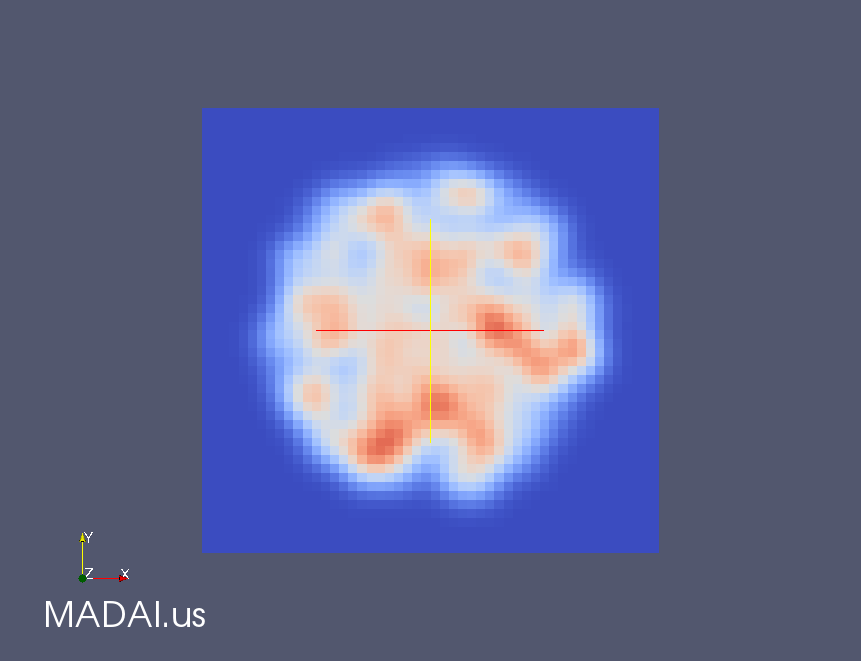
\includegraphics[scale=.25]{images/GaussianScalarSplatterPoint1.png} % requires the graphicx package
   \caption{Point density produced by the \textbf{GaussianScalarSplatter} filter (\texttt{NumberDensity} field) with standard deviation 0.1.}
   \label{fig:GaussianScalarSplatter1}
\end{figure}

Now change the \textbf{Standard Deviation} value to 0.2 and click \textbf{Rescale}. Notice how the splatted result is smoother.

\begin{figure}[htbp]
   \centering
   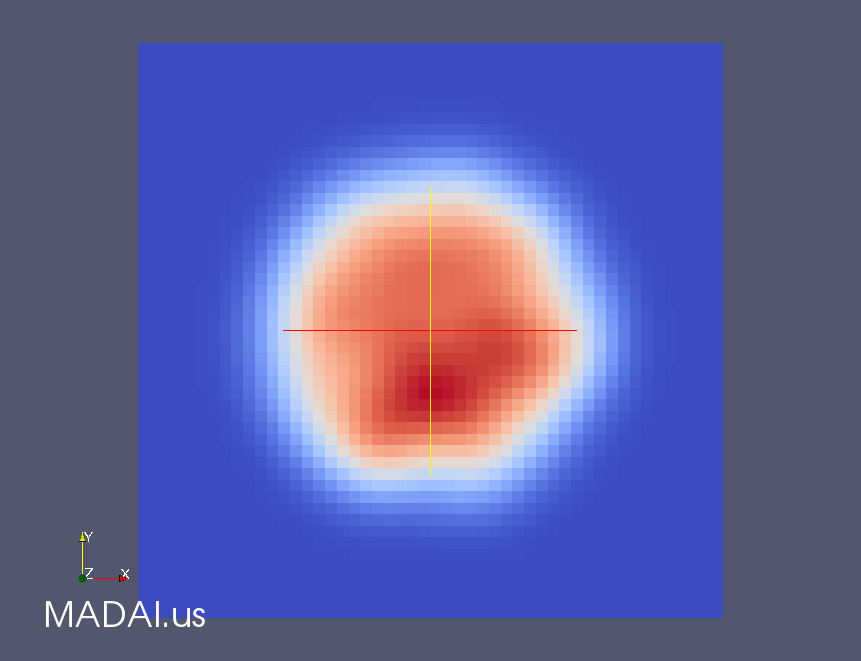
\includegraphics[scale=.25]{images/GaussianScalarSplatterPoint2.png} % requires the graphicx package
   \caption{Smoother point density produced by the \textbf{GaussianScalarSplatter} filter with standard deviation 0.2.}
   \label{fig:GaussianScalarSplatter2}
\end{figure}

Now color the slice by the \texttt{X\_Density} dataset and click the \textbf{Rescale} button.

\begin{figure}[htbp]
   \centering
   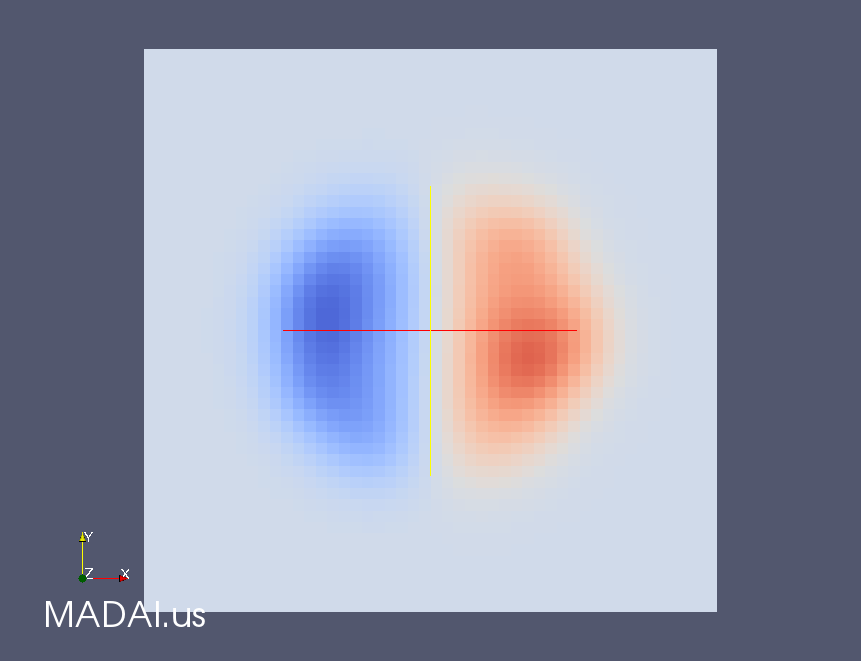
\includegraphics[scale=.25]{images/GaussianScalarSplatterXDensity.png} % requires the graphicx package
   \caption{\texttt{X\_Density} produced by the \textbf{GaussianScalarSplatter} filter with standard deviation 0.2.}
   \label{fig:GaussianScalarSplatter2}
\end{figure}


\bibliographystyle{plain}
\bibliography{MADAIWorkbenchTutorial}

\end{document}